\documentclass[10pt,a4paper]{article}

\usepackage[utf8]{inputenc}
\usepackage{graphicx}
\usepackage{gensymb}
\usepackage{amsmath}
\usepackage{amssymb}
\usepackage{geometry}
\usepackage{multicol}  
\usepackage{siunitx}
\usepackage{float}
\usepackage{color}
\graphicspath{{../figures/}}

\geometry{a4paper}

\author{Nik Dennler \\ Johannes Lade}
\title{Handout Digital Electronics Lab}
\date{\today{}}


\begin{document}
	
\begin{titlepage}
	\maketitle
		\begin{center}
			Email: nik.dennler@uzh.ch, johannes.lade@uzh.ch
		\end{center}
	\thispagestyle{empty}
\end{titlepage}



% \section{Construction of a combinatoric circuit}
% \begin{enumerate}
% 	\item Write down the truth table.
% 	\item Construct the disjunctive normal form from your truth table.
% 	\item Draw the circuit accordingly.
% 	\item Transform the circuit in such a way that it only uses NAND Gates.
% 	      How many NAND gates do you need? See if you can loose one or two gates.
% 	\item Check/discuss the circuit design again. An effective method is to create the truth table again just by looking at the circuit, then compare with what you should get. 
% 	\item If you're sure that your design works, build up the circuit with real components and connections. 
% \end{enumerate}

\newpage
\section{Boolean Logic}
\label{sec:exercise-block-1}

\subsection{Logic Symbols}


    \begin{figure}[H]
      \centering
      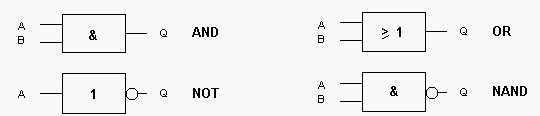
\includegraphics[width=1\textwidth]{gatter}%
      \caption{Logic Gatter}%
      \label{fig:gatter}
    \end{figure}
    
%\subsection{Elements explained}
    
%\begin{itemize}
%  \item \textbf{The conjunction (AND):} $a\land b$ is $1$ if and only if $a$ is $1$ and $b$ is $1$.\\
%  \item \textbf{The disjunction (OR):} $a\lor b$  is $1$ if and only if $a$ is $1$ or $b$ is $1$ or both.\\
%  \item \textbf{The negation (NOT):}  $\overline{a}$ is $1$ if and only if $a$ is $0$. \\
%  \item \textbf{The negated conjunction (NAND):}  $\overline{a}$ is $1$ if and only if $a$ is $0$.
  
%\end{itemize}

\subsection{Truth Table}

\begin{table}[H]
\centering
  \begin{tabular}{c|c||c|c|c|c}
  \textbf{$a$} & \textbf{$b$} & \textbf{$a\land b \ (AND)$} & \textbf{$a\lor b\ (OR)$} & \textbf{$\overline{a}\ (NOT a)$}  & \textbf{ {$\overline{a\land  b}\ (NAND)$}} \\ \hline
  0          & 0          & 0            & 0            & 1                & 1      \\
  0          & 1          & 0            & 1            & 1                & 1  \\
  1          & 0          & 0            & 1            & 0                & 1   \\
  1          & 1          & 1            & 1            & 0                & 0  
  \end{tabular}
\caption{truth table}
\label{tab:truth}
\end{table}

\section{NAND Conversion}
\subsection{Rules}
Every circuit, and especially each of the basic elements, can be built up by NAND's. The conversions can be figured out by comparing the Truth tables of various element combinations with the one from the NAND. They look as follows: 

    \begin{figure}[H]
      \centering
      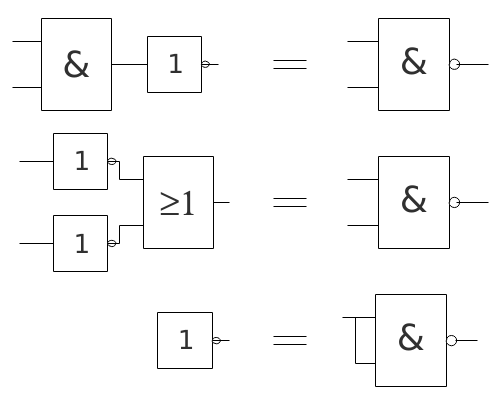
\includegraphics[width=0.4\textwidth]{nand_conversion}%
      \caption{NAND Conversion}%
      \label{fig:nand_conversion}
    \end{figure}

Also important is the realization, that two negations right after each other do not change anything!

\subsection{Procedure}
Let's convert the equivalence circuit to NAND's only. 
\begin{enumerate}
 \item Draw the circuit as in the disjunctive normal-form.
     \begin{figure}[H]
      \centering
      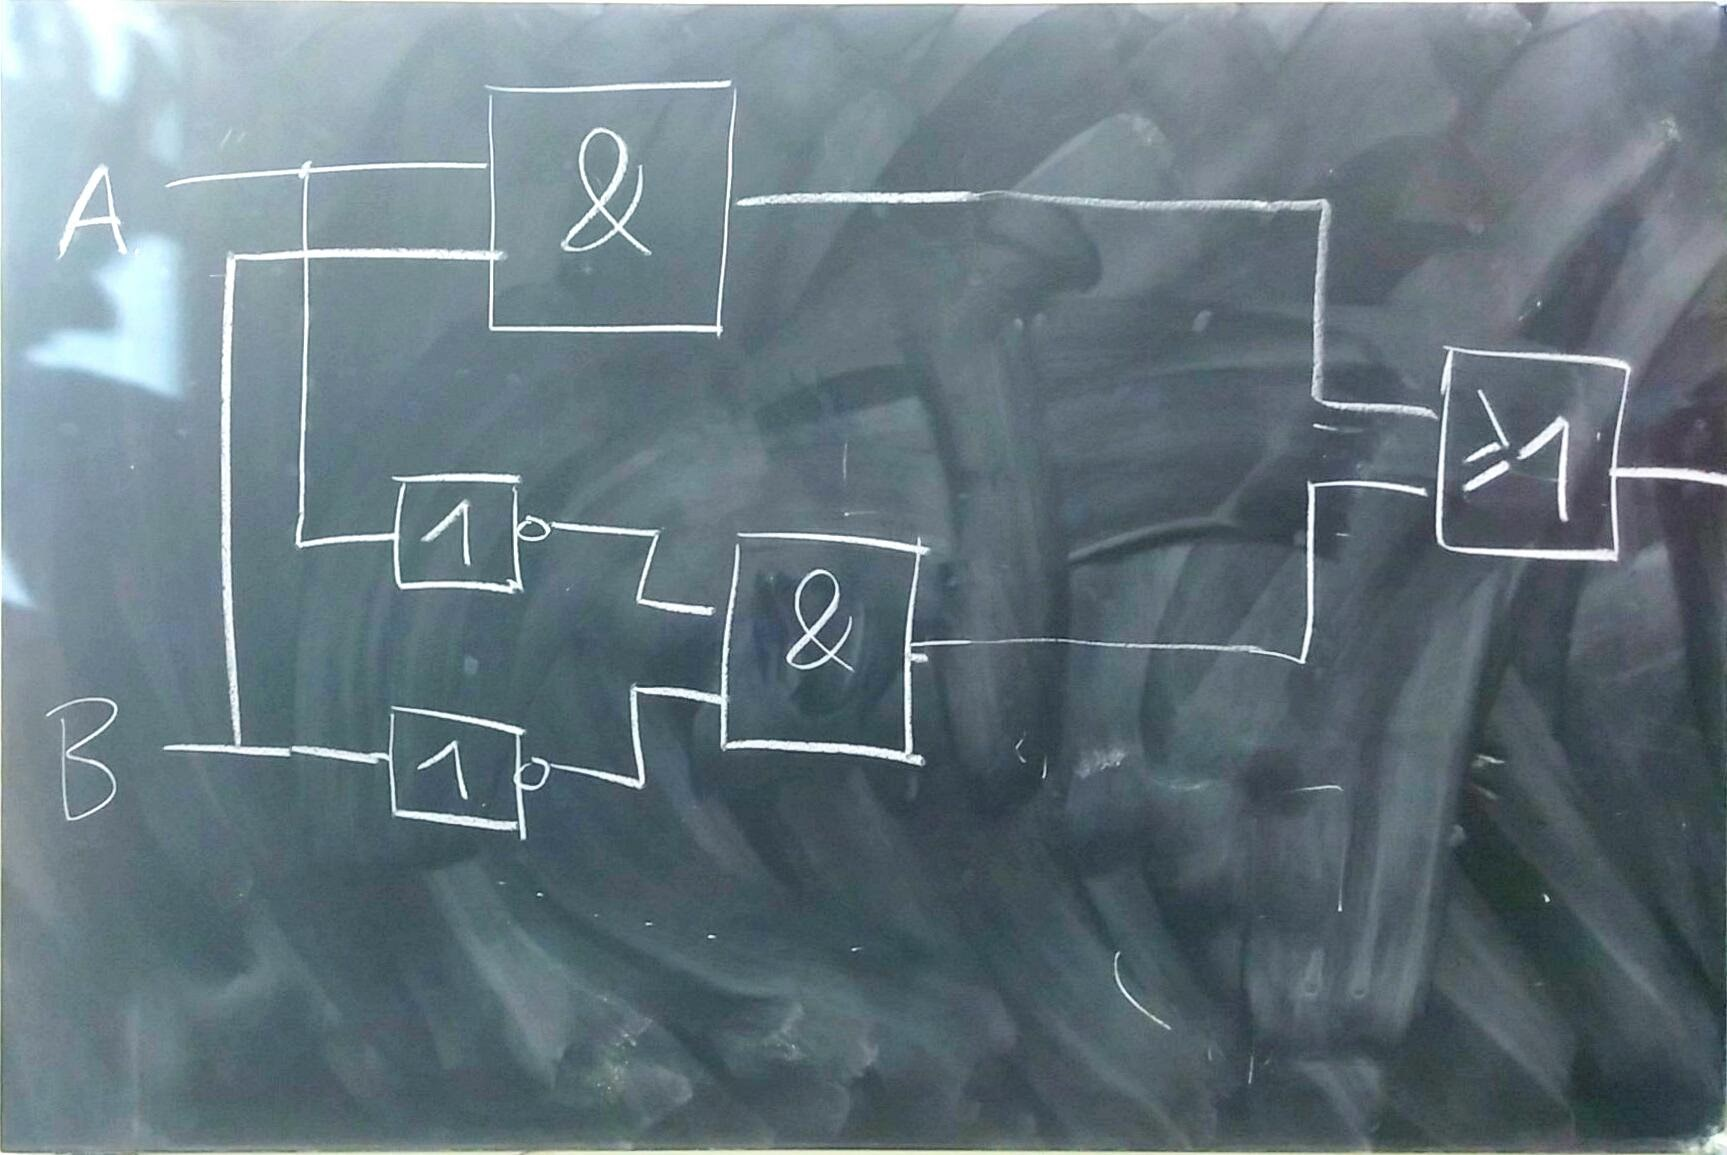
\includegraphics[width=0.4\textwidth]{eq1}%
      \caption{Equivalence circuit}%
      \label{fig:eq1}
    \end{figure}
 \item Plug in the double inversion anywhere where it could make sense. See the patterns according to the conversion rules.
      \begin{figure}[H]
      \centering
      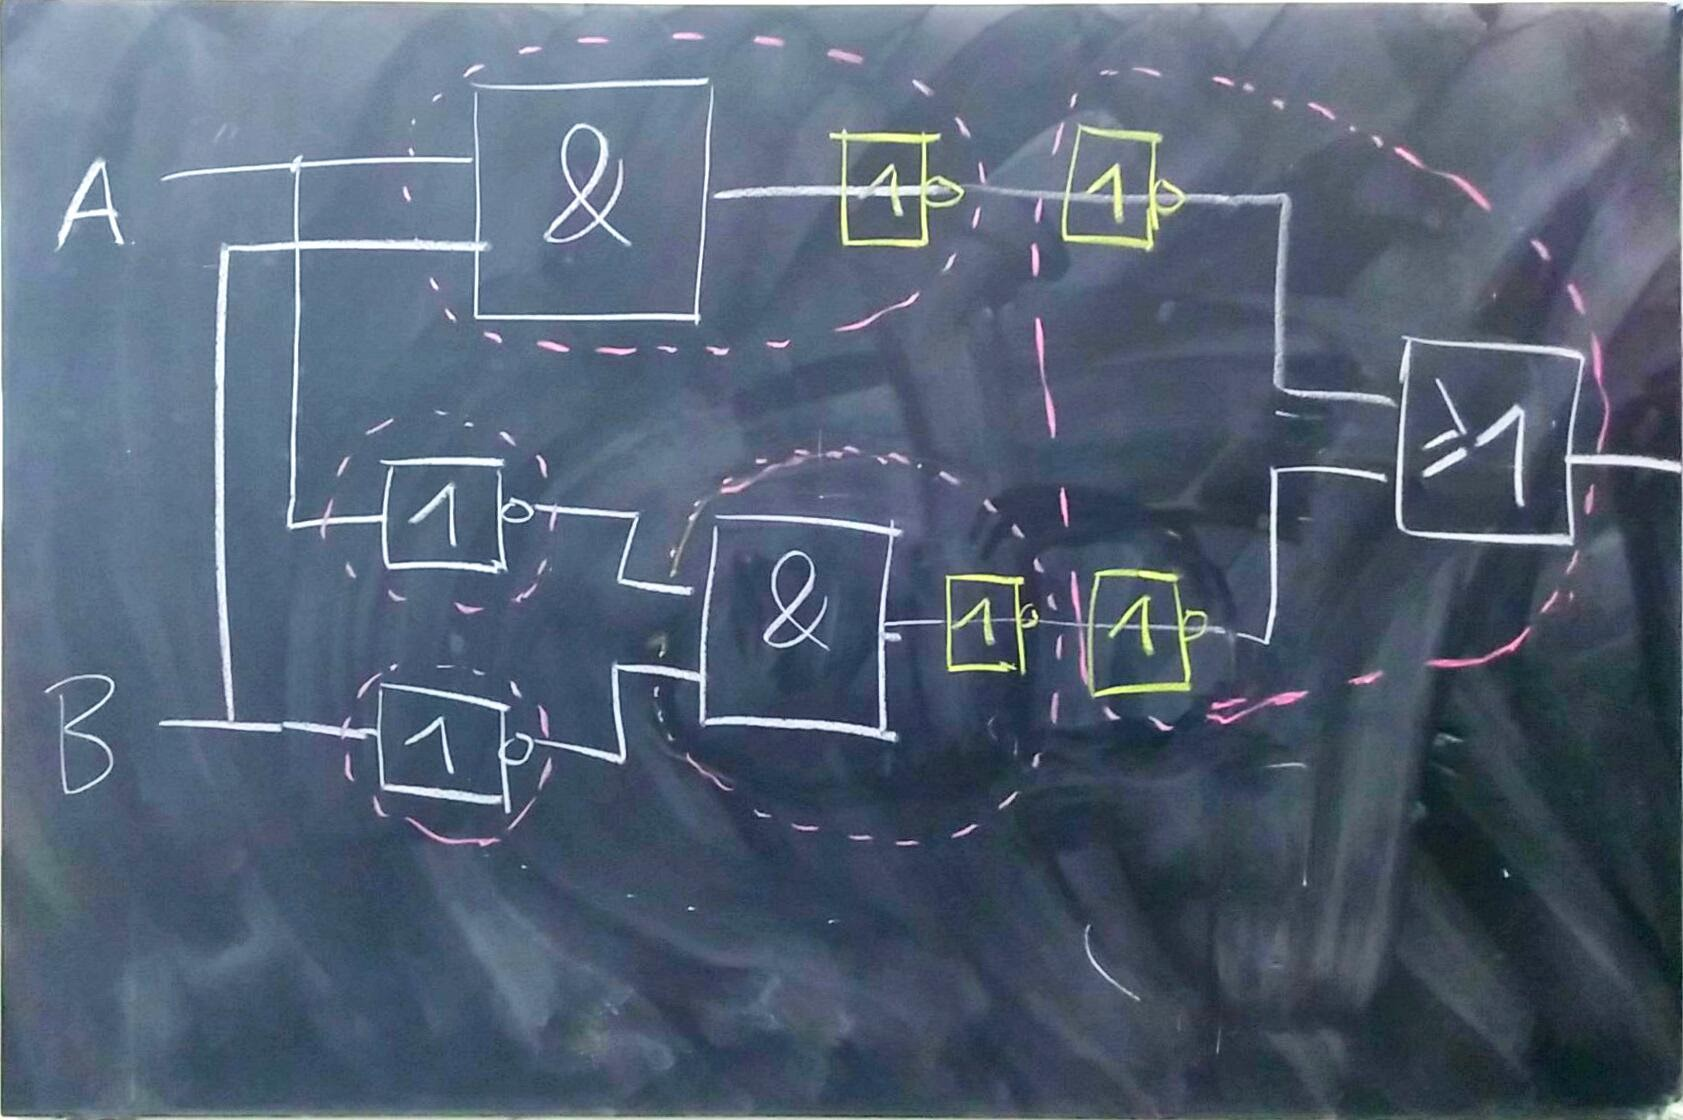
\includegraphics[width=0.4\textwidth]{eq2}%
      \caption{Equivalence circuit with added double inversions}%
      \label{fig:eq2}
    \end{figure}
 \item Now draw the circuit again with NAND gates only.
      \begin{figure}[H]
      \centering
      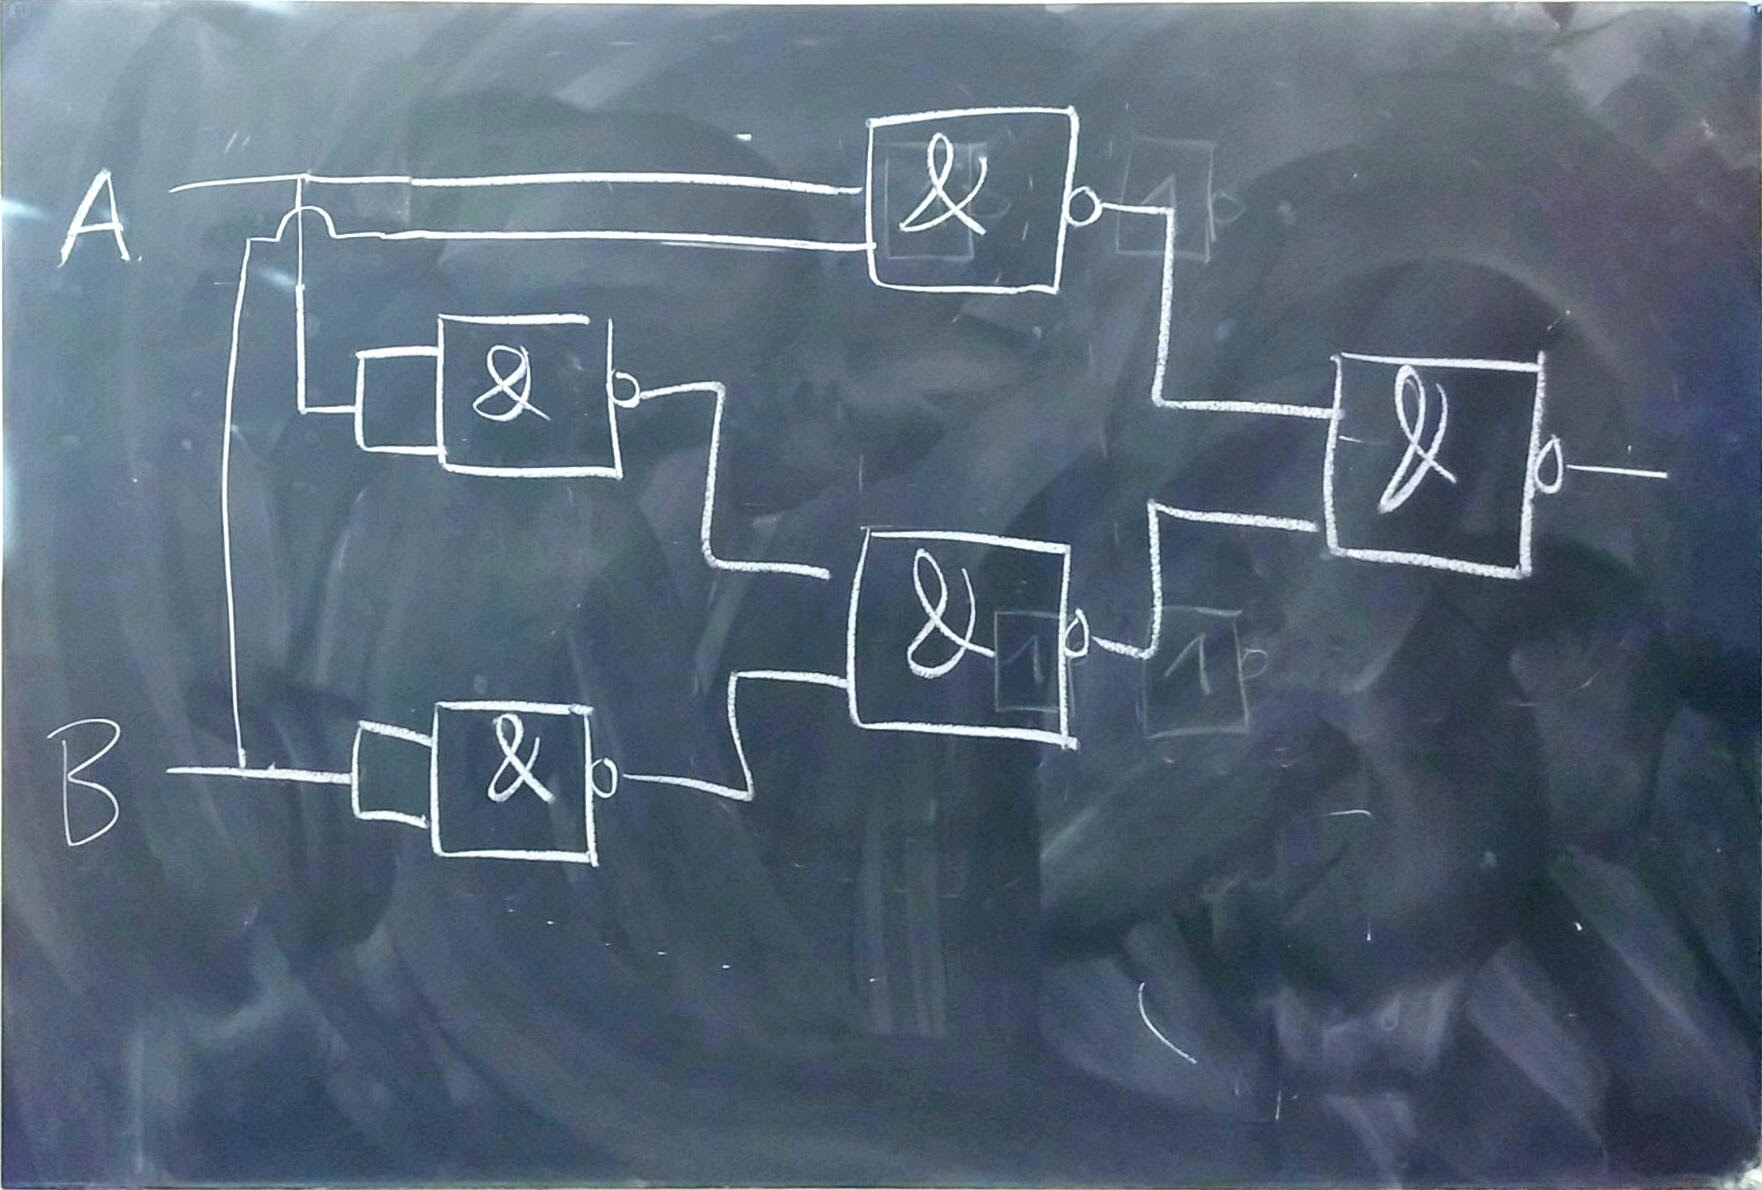
\includegraphics[width=0.4\textwidth]{eq3}%
      \caption{Equivalence circuit with NANDs only}%
      \label{fig:eq3}
    \end{figure}
\end{enumerate}





\newpage

\section{Hardware}

\subsection{Breadboard}
Let's look at the breadboard design.
    \begin{figure}[H]
      \centering
      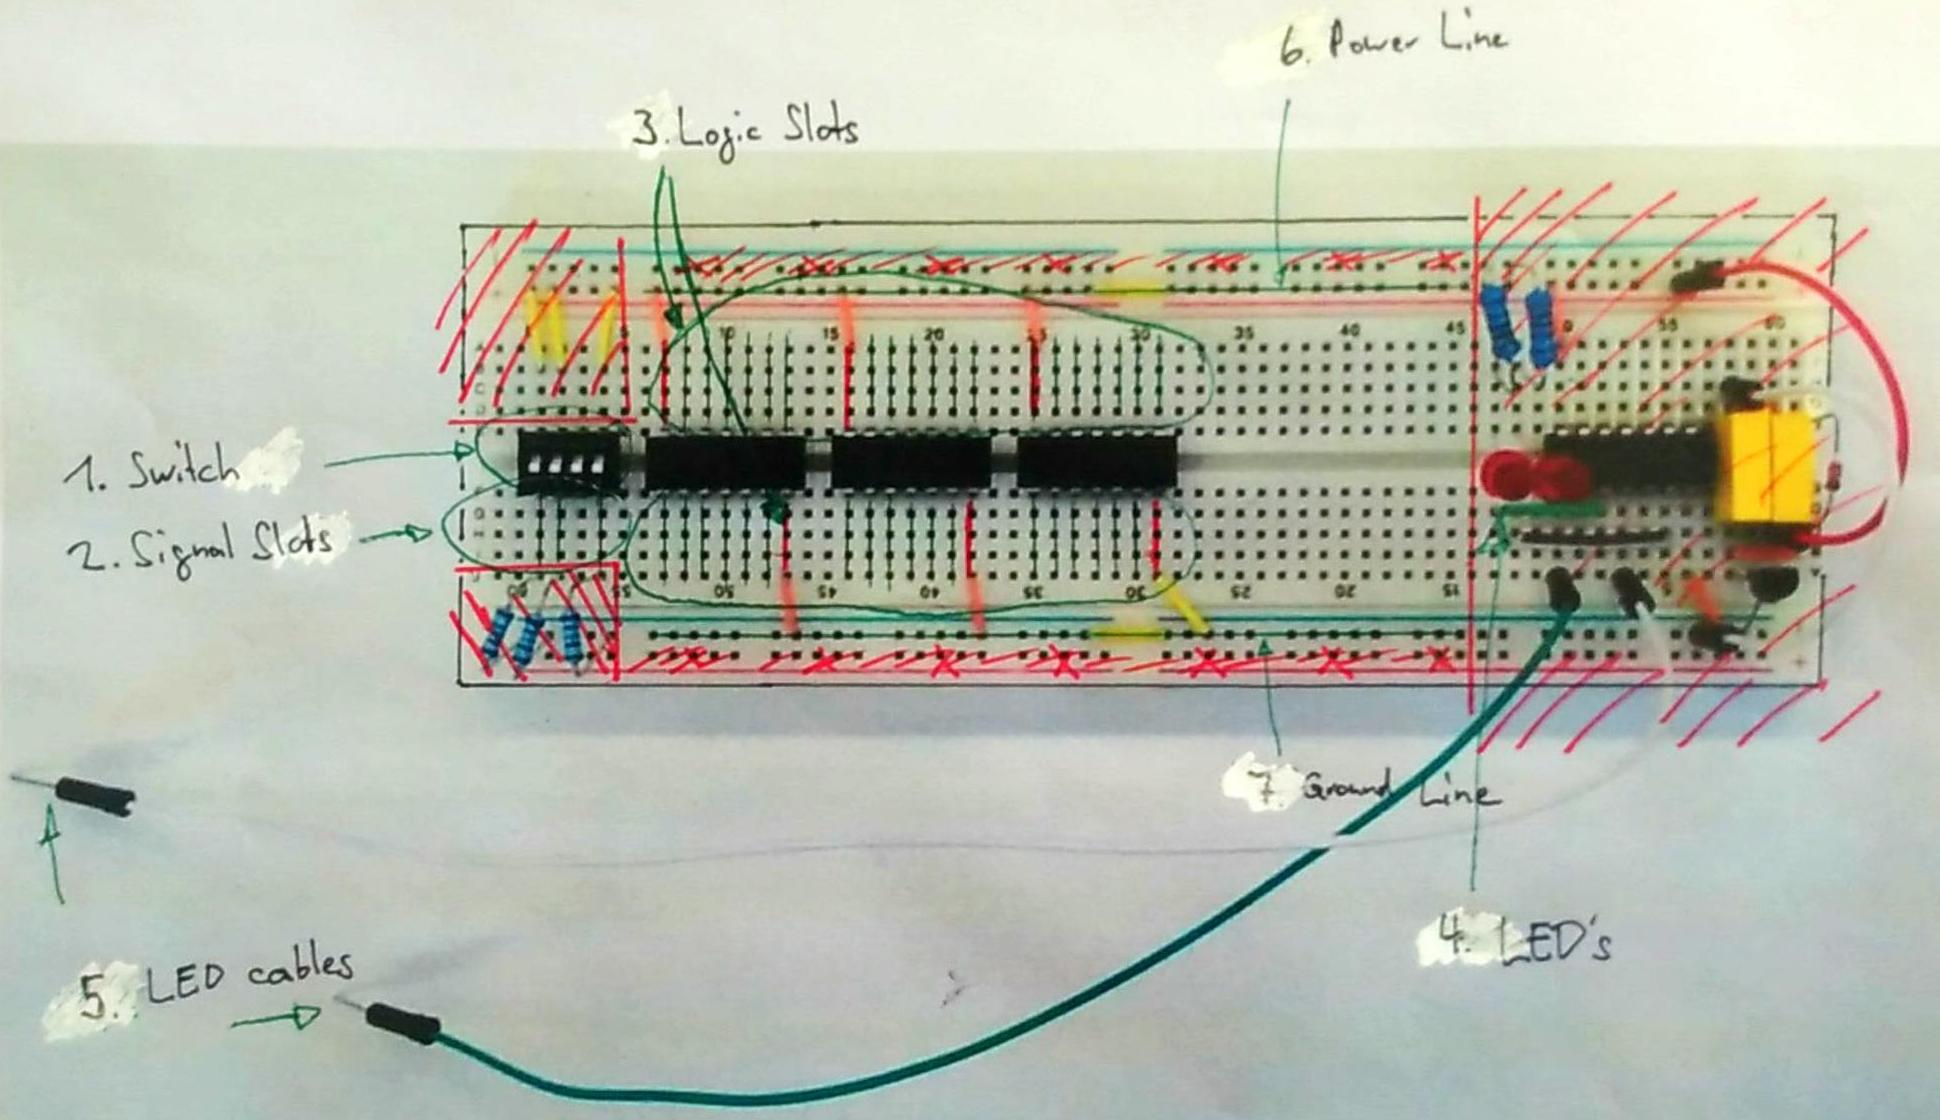
\includegraphics[width=0.9\textwidth]{breadboard_labeled}%
      \caption{Breadboard}%
      \label{fig:breadboard_labelled}
    \end{figure}

\begin{enumerate}
 \item The input switch can be set to \texttt{1} (up) or \texttt{0} (down). Try to hold the part while switching, else it might fall out of the board!
 \item On the signal slots you can plug in a jumper cable and connect the signal to wherever you want it.
 \item On the logic slots, you can connect the in- and outputs of your NAND-gates with each other and with the signal and LED's. 
 \item The loose cables are connected to the LED's. Plug them in wherever you want to test something.
 \item The LED's help you to understand your output signals. Attention: They light up if they're plugged in to a \texttt{1} \underline{or if they're not connected to anything at all}. 
 \item The red power line is connected to the \texttt{+} of the power source.
 \item The blue groud line is connected to the \texttt{-} of the power source. 
\end{enumerate}


\newpage
\subsection{Chip (NAND-Gates)}
We use a SN7400N chip. They have a power pin, a ground pin, as well as four NAND-gates. The pins are occupied as shown below:
    \begin{figure}[H]
      \centering
      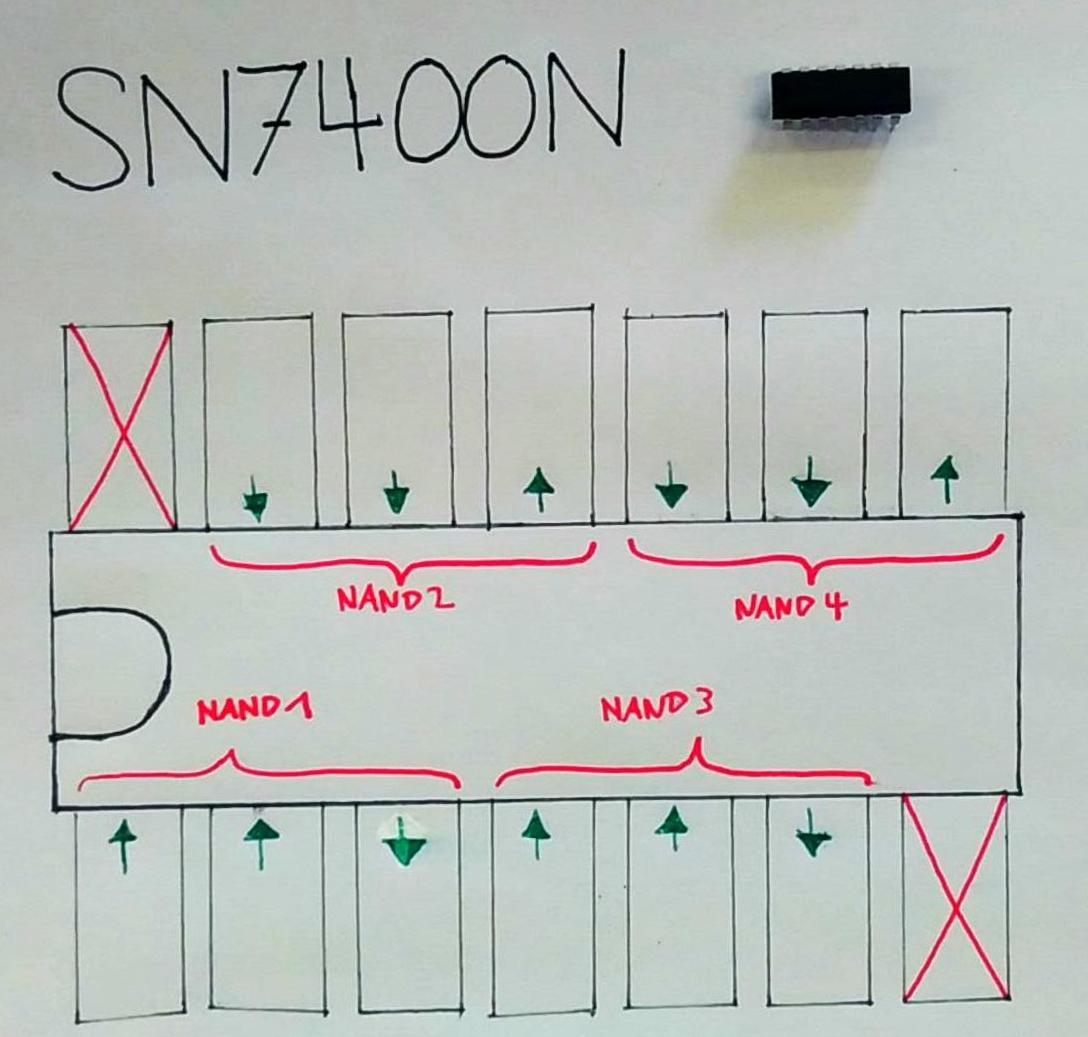
\includegraphics[width=0.6\textwidth]{sn7400n}%
      \caption{Chip with NAND-gates on it}%
      \label{fig:sn7400n}
    \end{figure}   


\end{document}



